\section{Entanglement in quantum mechanical system}\label{ss:BasicEE}

We introduce the notion of bipartite entanglement for pure states in finite-dimensional quantum mechanical systems and classify the states into two types depending on whether they contain nontrivial entanglement entropy that quantifies the amount of quantum entanglement.
A set of inequalities of entanglement entropy, which will play crucial roles in the latter sections, will be given without proofs.
Other entanglement measures frequently used in the literature will also be introduced and compared with entanglement entropy.



\subsection{Bipartite entanglement}
\label{ss:def EE}
Given a lattice model or QFT, suppose the system is in a
pure ground state $|\Psi\rangle$, i.e., 
the density matrix for the Hilbert space $\CH_\text{tot}$ is given in the form\footnote{We normalize the ground state as $\langle \Psi |\Psi\rangle = 1$ so that $\tr_\text{tot} (\rho_\text{tot}) = 1$.}
\begin{align}\label{pure}
\rho_\text{tot}=|\Psi\rangle \langle
\Psi| \ . 
\end{align}
We then divide the total system into two subsystems $A$ and $B = \bar A$ complementary to each other as in Fig.\ \ref{fig:spinchain}.
\begin{figure}[htbp]
\centering
	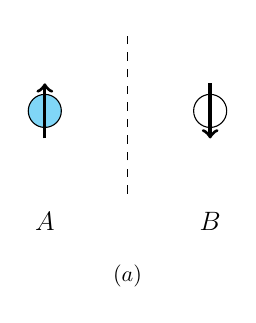
\begin{tikzpicture}[scale=.7, every node/.style={scale=0.8}]
		\draw[dashed] (0, -1.5) -- (0, 1.5);
		\filldraw[fill=cyan!50] (-1.5, 0) circle (0.3);
		\draw (1.5, 0) circle (0.3);
		\draw[very thick, ->] (-1.5, -0.5) -- (-1.5, 0.5);
		\draw[very thick, ->] (1.5, 0.5) -- (1.5, -0.5);
		\node at (-1.5, -2) {\large $A$};
		\node at (1.5, -2) {\large $B$};
		\node at (0, -3) {$(a)$};
	\end{tikzpicture}
	\qquad\qquad
	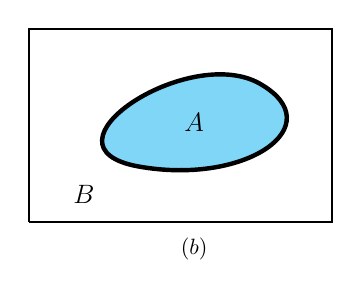
\begin{tikzpicture}[scale=.7, every node/.style={scale=.8}]
		\draw[thick] (-3,-2) -- (2.5, -2) -- (2.5, 1.5) -- (-3, 1.5) -- (-3, -2);
		\filldraw[ultra thick, fill=cyan!50] (-1, -1) .. controls +(170:2) and +(150:1.5) .. (1.2, 0.5) .. controls +(-30:1.5) and +(-10:2) .. (-1, -1);
		\node at (0,-0.2) {\large $A$};
		\node at (-2,-1.5) {\large $B$};
		\node at (0, -2.5) {$(b)$};
	\end{tikzpicture}
\caption{
\label{fig:spinchain}
The decomposition of the system into a subsystem $A$ shown in blue and its complement $B$.
$(a)$ Two spin systems. The subsystems $A$ and $B$ are left and right spins, respectively.
$(b)$ In $d$-dimensional quantum field theory, a spatial region at a given time slice is split into the subsystems $A$ and $B$ whose common boundary $\partial A = \partial B$ is always a codimension-two hypersurface in $d$ dimensions.
}
\end{figure}

In the spin chain example,
we cut off the chain in between the sites and divide the lattice points into two groups. 
Note that this cutting procedure is an imaginary process without changing the system at all.
In what follows, the total Hilbert space will be assumed to take a direct product form of two Hilbert spaces of the subsystems,\footnote{This assumption is not necessarily valid for QFTs in general, especially with gauge symmetries.
We, however, will ignore this issue for simplicity in the reminder of this review.
For discussions and attempts to define entanglement entropy in gauge theories, see, e.g., \textcite{Casini:2013rba,Radicevic:2014kqa,Donnelly:2014gva,Donnelly:2014fua,Huang:2014pfa,Ghosh:2015iwa,Hung:2015fla,Aoki:2015bsa,Chen:2015kfa,Donnelly:2015hxa,Radicevic:2015sza,Pretko:2015zva,Soni:2015yga,Ma:2015xes,VanAcoleyen:2015ccp} and a review by \textcite{Pretko:2018yxl}.
}
\begin{align}
	\CH_\text{tot} = \CH_{A}\otimes \CH_{B} \ .
\end{align}

Let $\{ |i\rangle_B, i=1,2,\cdots\}$ be an orthonormal basis in $\CH_B$, and define
the {\it reduced density matrix} $\rho_A$ of the system $A$ by taking the partial trace over the system $B$,
\begin{align}\label{ReducedDM}
\rho_A \equiv \tr_{B}( \rho_\text{tot} ) \equiv \sum_{i} {}_B\langle i |\, \rho_\text{tot} \,| i\rangle_B \ .
\end{align}
Note that this definition depends on the choice of the subsystem, but not on the choice of the orthonormal basis $\{ |i\rangle_B\}$.
For example, if $\rho_\text{tot}$ is the tensor product of the density matrices $\rho_A$ and $\rho_B$ describing the subsystems, $\rho_\text{tot} = \rho_A \otimes \rho_B$, the partial trace simply recovers them, $\tr_B(\rho_\text{tot}) = \rho_A$ and $\tr_A(\rho_\text{tot}) = \rho_B$.

An alternative characterization of the reduced density matrix is the condition
\begin{align}
	\tr\left(\rho_\text{tot}\, \CO \right) = \tr_A\left( \rho_A \,\CO_A\right)\ ,
\end{align}
for any operator $\CO$ of the form $\CO = \CO_A \otimes {\bf 1}_B$ with the identity operator ${\bf 1}_B$ in $\CH_B$.
In this sense, the reduced density matrix $\rho_A$ has enough information for $\CH_A$ to reconstruct every correlation function in the subregion $A$.
The total density matrix needs not be pure in this characterization, but one may wonder, once the complete information $\rho_A$ about a system $A$ is given, if it is possible to find a pure density matrix in an enlarged Hilbert space of $\CH_A$ whose partial trace recovers $\rho_A$.
Indeed the answer is affirmative, and one can always construct such an enlarged Hilbert space and the density matrix in the following way.
The most general density matrix is of the form
\begin{align}
	\rho_A = \sum_i\, p_i\, |i\rangle_A {}_A\langle i | \ ,
\end{align}
where $\{ |i\rangle_{\bar A} \}$ is an orthonormal basis of $\CH_A$ and the coefficients $p_i \ge 0$ sum up to $1$, $\sum_i \,p_i = 1$.
We then copy $\CH_A$ into another Hilbert space $\CH_{\bar A}$ with the basis given by $\{ |i\rangle_{\bar A} \}$ and define a pure density matrix $\rho$ by
\begin{align}\label{Def_Purification}
	\rho = |\chi\rangle \langle \chi| \ , \qquad |\chi\rangle \equiv \sum_{i}\, \sqrt{p_i} \, |i\rangle_A \otimes | i \rangle_{\bar A} \ ,
\end{align}
in the enlarged Hilbert space $\CH = \CH_A\otimes \CH_{\bar A}$.
It is straightforward to check that this construct correctly reproduces $\rho_A$ under the partial trace over $\bar A$.
The operation is called \emph{entanglement purification} as it constructs a pure unentangle state from a mixed entangled state by enlarging the Hilbert space.
In Sec. \ref{ss:RindlerTFD}, we see that the entanglement purification turns out to be a fundamental concept in understanding what an observer restricted to a subregion feels like in a thermal system in QFT.

Finally let us introduce a measure of entanglement, the {\it entanglement entropy} of the subsystem $A$, by the von Neumann entropy of the reduced density matrix $\rho_A$,
\begin{align}\label{EE_def}
S_A =
- \mathrm{tr}_{A}\left[
\rho_{A} \log \rho_{A}\right] \ .
\end{align}
Note that the entanglement entropy of the total system always vanishes, $S_\text{tot} = 0$ for a pure ground state \eqref{pure}. 
Entanglement entropy remains finite in a finite-dimensional quantum system, but it suffers from UV divergences in QFT due to the short range interaction near the boundary $\partial A$ of the subsystem $A$ as discussed in detail in Sec. \ref{ss:Euclidean}.


\subsection{Separable and entangled states}
Having introduced a notion of entanglement entropy as the von Neumann entropy of the density matrix of a subsystem $A$, we want to understand what it really measures for a given system.
To proceed with the discussion, consider a pure ground state $|\Psi\rangle$ in a general form:
\begin{align}\label{PureProductState}
|\Psi\rangle = \sum_{i,\mu} c_{i\mu}\, |i\rangle_A  \otimes |\mu \rangle_B  \ ,
\end{align}
where $|i\rangle_A$ and $|\mu\rangle_B$ are orthonormal bases for $\CH_A = \{ |i\rangle_A, i = 1, \cdots, d_A\}$ and $\CH_B = \{ |\mu\rangle_B, \mu = 1, \cdots, d_B\} $, respectively, and the coefficient $c_{i\mu}$ is a $d_A \times d_B$ matrix with complex entries.
There are two different cases depending on the type of the coefficient matrix $c_{i\mu}$.


\subsubsection{Separable state}
When $c_{ij}$ factorizes, $c_{ij} = c_i^A c_\mu^B$, the ground state $|\Psi\rangle$ is called a \emph{separable} state (a pure product state) and can be recast into the product form,
\begin{align}
|\Psi\rangle = |\Psi_A \rangle \otimes |\Psi_B\rangle \ , 
\end{align}
where $|\Psi_{A} \rangle \equiv \sum_i c_i^{A} |i\rangle_{A}$ and $|\Psi_{B} \rangle \equiv \sum_\mu c_\mu^{B} |\mu\rangle_{B}$.
This is the case where the reduced density matrix, Eq.\,\eqref{ReducedDM}, also becomes pure $\rho_A = |\Psi_A\rangle\langle\Psi_A|$.
Thus a separable state has vanishing entanglement entropy
\begin{align}
	S_A = 0 \ .
\end{align}
Moreover, one can show entanglement entropy vanishes if and only if the pure ground state is separable as we will see.


\subsubsection{Entangled state} 
The ground state is called an {\it entangled} (or inseparable) state if it is not separable (with the coefficient matrix $c_{i\mu} \neq c_i^A c_\mu^B$).
This is the case where the entanglement entropy takes a positive value.

Indeed, we can simplify Eq.\,\eqref{PureProductState} by changing the bases into the \emph{Schmidt decomposition} form,
\begin{align}\label{PureDiag}
|\Psi\rangle = \sum_{k=1}^{\text{min}(d_A, d_B)} \sqrt{p_k}\, |\psi_k\rangle_A\otimes  |\psi_k \rangle_B \ ,
\end{align}
where $p_k$ are non-negative real numbers satisfying $\sum_k p_k = 1$ and
$|\psi_k\rangle_{A,B} $ are new orthonormal bases for the subsystems $A$ and $B$.
Note that this decomposition works for any $d_A \times d_B$ rectangular matrix $c_{i\mu}$.
To see how it actually works, we ``diagonalize" the coefficient matrix by the singular-value decomposition,
\begin{align}
c = U \, \Sigma\, V^\dagger \ ,
\end{align}
where $U$ and $V$ are $d_A \times d_A$ and $d_B\times d_B$ unitary matrices.
$\Sigma$ is a diagonal $d_A\times d_B$ real matrix given by
\begin{align}
	\Sigma = 
		\begin{cases}
			\left(\begin{array}{ccc|c}
			\sqrt{p_1} & & &  \\
			& \ddots & & \bf 0 \\
			& & \sqrt{p_{d_B}} & 
			\end{array}\right)  &\qquad  (d_A < d_B) \ , \\
			\\
			\left(\begin{array}{ccc}
			\sqrt{p_1} & &  \\
			& \ddots &  \\
			& & \sqrt{p_{d_A}}\\
			\hline
			 & \bf 0 &
			\end{array}\right) &\qquad  (d_A \ge d_B) \ , 
		\end{cases}
\end{align}
with non-negative real entries $\sqrt{p_k}\ge 0$, $k=1,\cdots, \text{min}(d_A, d_B)$.
The square root for the eigenvalues is purely conventional for later use.
The new orthonormal bases  $|\psi_k\rangle_{A,B}$ are the unitary transformation of the original ones $|i\rangle_{A,B}$ as $|\psi_k\rangle_A = \sum_{i} U_{ik} |i\rangle_A$ and $|\psi_k\rangle_B = \sum_{\mu} V_{k\mu} |\mu\rangle_B$.

The Schmidt decomposition Eq.\,\eqref{PureDiag} is particularly nice as it yields a mixed state density matrix with the probability distribution $\{ p_k\}$ for the reduced density matrix,
\begin{align}\label{Red_DM_A}
\begin{aligned}
	\rho_A &= \sum_{i=1}^{d_B} {}_B\langle \psi_i | \Psi \rangle \langle \Psi | \psi_i \rangle_B \ ,\\
		&= \sum_{k=1}^{\text{min}(d_A, d_B)}\, p_k\, |\psi_k\rangle_A\, {}_A\langle \psi_k | \ .
\end{aligned}
\end{align}
In our case, the condition $\sum_k\, p_k = 1$ follows from the normalization $\langle \Psi |\Psi\rangle = 1$.
We see that the reduced density matrix of a subsystem can be mixed even if the total system is in a pure ground state.
This should be compared with the discussion for entanglement purification around Eq.\,\eqref{Def_Purification} where we saw the opposite.
In the Schmidt decomposition the entanglement entropy 
\begin{align}\label{SchmidtEE}
S_A = - \sum_{k=1}^{\text{min}(d_A, d_B)} p_k \,\log p_k
\end{align}
is nothing but the Shannon entropy of the probability distribution $\{ p_k\}$.
Under the constraint $\sum_k p_k = 1$, it takes the maximum value
\begin{align}\label{MES}
S_A|_\text{max} = \log \text{min}(d_A, d_B)
\end{align}
at $p_k = 1/\text{min}(d_A, d_B)$ for any $k$.\footnote{To prove Eq.\,\eqref{MES}, one can introduce the Lagrange multiplier $x\,(\sum_{k}p_k -1)$ to the entropy Eq.\,\eqref{SchmidtEE} and extremize it with respect to $p_k$.}


\bigskip
In summary, an entangled state is a superposition of several quantum states.
An observer who can  access only a subsystem $A$ will find him or herself in a mixed state when the pure ground state $|\Psi\rangle$ in the total system is entangled:
\begin{align}
\begin{aligned}
	 |\Psi\rangle:& ~\text{separable} \qquad &\longleftrightarrow \qquad &\rho_A: \text{pure state} \ , \\
	 |\Psi\rangle:& ~\text{entangled} \qquad &\longleftrightarrow \qquad &\rho_A: \text{mixed state} \ .
\end{aligned}
\end{align}

Entanglement entropy measures how much a given state differs from a separable state.
It reaches the maximum value when a given state is a superposition of all possible quantum states with an equal weight. 



\paragraph{Two spin system}\label{TwoSpin}
Let us illustrate a simple example of an entangled state.
Consider a system of two particles $A$ and $B$ with spin $1/2$.
The Hilbert spaces $\CH_A$ and $\CH_B$ are spanned by two states: $\CH_{A,B} = \{ |0\rangle_{A,B}, |1\rangle_{A,B}\}$.
We let them be orthonormal bases satisfying ${}_{A,B}\langle i | j \rangle_{A,B} = \delta_{ij}$ for $i,j = 0,1$.
Since the total Hilbert space is the tensor product of the two subsystems $\CH_\text{tot} = \CH_A \otimes \CH_B$, it has the four-dimensional orthonormal basis: $\CH_\text{tot} = \{ |00\rangle, |01\rangle, |10\rangle, |11\rangle \}$ where $|ij\rangle \equiv |i\rangle_A \otimes |j\rangle_B$ are tensor product states.

Suppose the ground state is given by
\begin{align}\label{TwoSpinPure}
|\Psi\rangle = \frac{1}{\sqrt{2}} \Big( |01\rangle - |10\rangle \Big) \ .
\end{align}
The reduced density matrix for the particle $A$ is obtained by taking the partial trace over $\CH_B$ of the total density matrix Eq.\,\eqref{pure}, 
\begin{align}
\begin{aligned}
	\rho_A &=  \frac{1}{2}\Big( |0\rangle_A \,{}_A\langle 0 |   +  |1 \rangle_A \,{}_A\langle 1 |\Big) \ .
\end{aligned}
\end{align}
It is convenient to write it in a matrix form acting on the two-dimensional vector space $\CH_A$,
\begin{align}\label{TwoSpinRD}
	\rho_A = \left( 
		\begin{array}{cc}
			1/2 & 0 \\
			0 & 1/2
		\end{array}
		\right) \ .
\end{align}
It shows that $\rho_A$ is not pure and 
the entanglement entropy does not vanish,
\begin{align}\label{EE_TwoSpin}
\begin{aligned}
S_A &= -\tr_A \left[ \left( 
		\begin{array}{cc}
			1/2 & 0 \\
			0 & 1/2
		\end{array}
		\right)  \left( 
		\begin{array}{cc}
			\log(1/2) & 0 \\
			0 & \log(1/2)
		\end{array}
		\right)    \right] \ , \\
	&=\log 2 \ .
\end{aligned}
\end{align}
This is a maximally entangled state for it saturates the upper bound Eq.\,\eqref{MES} with $d_A = d_B = 2$.


A more general state to consider is
\begin{align}
|\Psi\rangle =  \cos\theta\, |0 1 \rangle - \sin\theta\, |10\rangle \ ,
\end{align}
parametrized by a parameter $\theta$ ranging from $0$ to $\pi/2$, that reduces the state Eq.\,\eqref{TwoSpinPure} at $\theta=\pi /4$.
By a similar calculation we have
\begin{align}
	S_A = - \cos^2 \theta \log ( \cos^2 \theta) - \sin^2\theta \log (\sin^2\theta) \ ,
\end{align}
which shows the states at $\theta = 0, \pi /2$ are pure product states with vanishing entanglement entropy while the state Eq.\,\eqref{TwoSpinPure} at $\theta= \pi/4$ is maximally entangled.


\paragraph{Thermofield double state}
A more nontrivial example of an entangled state is the thermofield double state defined by
\begin{align}\label{TFD}
	| \Psi\rangle = \frac{1}{\sqrt{Z} }\sum_n\,e^{-\beta E_n/2} |n\rangle_A \otimes |n\rangle_B \ ,
\end{align}
where we normalize the state with the partition function $Z = \sum_n e^{-\beta E_n}$.
The peculiarity of the thermofield double state becomes manifest in taking the partial trace over the subsystem $B$.
Namely the reduced density matrix for the subsystem $A$ becomes a Gibbs state of inverse temperature $\beta$:
\begin{align}\label{Gibbs_State}
\begin{aligned}
	\rho_A  &=  \frac{1}{Z} \sum_{n} e^{-\beta E_n} |n\rangle_A {}_A\langle n | \ ,\\
		&= \frac{1}{Z}\, e^{-\beta H_A} \ .
\end{aligned}
\end{align}
In the second line, we introduced the (modular) Hamiltonian $H_A$ such that $H_A |n\rangle_A = E_n |n\rangle_A$.
Actually the thermofield double state is the entanglement purification of a thermal state with the Boltzmann weight $p_i = e^{-\beta\,E_i}/Z$ in Eq.\,\eqref{Def_Purification}.
Namely we can purify the thermal system $A$ in the extended Hilbert space $\CH_A\otimes \CH_B$ by copying the state vectors $\{ |n\rangle_B\}$ from $\CH_A$ to $\CH_B$.
Then every expectation value of local operators in the thermal system $A$ is representable in the thermofield double state Eq.\,\eqref{TFD} of the total system $A\cup B$.
In this example, the entanglement entropy measures the thermal entropy of the subsystem $A$:
\begin{align}
\begin{aligned}
	S_A &= -\tr_A\left[ \rho_A\, (-\beta H_A - \log Z)\right] \ , \\
		&= \beta \,(\langle H_A \rangle -F)   \ ,
\end{aligned}
\end{align}
where $F$ is the thermal free energy $\beta\, F = - \log Z$.

The thermofield double state is also important to understand the thermal nature of black holes when we consider QFT on a background geometry with a horizon in Sec. \ref{ss:RindlerTFD}.




\subsection{Bell states}
In the two spin system, we saw the state Eq.\,\eqref{TwoSpinPure} is maximally entangled.
Actually there are totally four independent maximally entangled states in the two qubit system:
\begin{align}\label{BellStates}
\begin{aligned}
	|B_1\rangle &= \frac{1}{\sqrt{2}} \Big( |00\rangle + |11\rangle\Big) \ ,\\
	|B_2\rangle &= \frac{1}{\sqrt{2}} \Big(  |00\rangle - |11\rangle\Big) \ ,\\
	|B_3\rangle &= \frac{1}{\sqrt{2}} \Big(  |01\rangle + |10\rangle\Big) \ ,\\
	|B_4\rangle &= \frac{1}{\sqrt{2}} \Big(  |01\rangle - |10\rangle\Big) \ .
\end{aligned}
\end{align}
These are known as the Bell states or Einstein-Podolsky-Rosen pairs in quantum information theory.
These states manifest their quantum mechanical aspects in the sense that they violate the Bell's inequalities holding in a local hidden variable theory accounting for the probabilistic features of quantum mechanics with a hidden variable and a probability density. 


For a system of $n$ qubits, there are entangle states called the Greenberger-Horne-Zeilinger (GHZ) states \cite{greenberger1989going,greenberger1990bell}:
\begin{align}
	|\text{GHZ}\rangle = \frac{1}{\sqrt{2}} \left( |0\rangle^{\otimes n} + |1\rangle^{\otimes n} \right) \ .
\end{align}
Another type of entangled states is called the $W$ state \cite{Dur:2000zz},
\begin{align}
	|W \rangle = \frac{1}{\sqrt{n}} \left( |10\cdots00\rangle +  |010\cdots 0\rangle +\cdots + |00\cdots01\rangle  \right) \ .
\end{align}
These two types of states are inequivalent as the GHZ state is fully separable while the $W$ state is not as seen next.


\paragraph*{Tripartite system $:$}
In a tripartite system ($n=3$), the GHZ and $W$ states become
\begin{align}\label{GHZstate}
	|\text{GHZ}\rangle = \frac{1}{\sqrt{2}} \left( |000\rangle + |111\rangle \right) \ ,
\end{align}
and 
\begin{align}
	|W\rangle = \frac{1}{\sqrt{3}} \left( |001\rangle + |010\rangle + |100\rangle\right) \ .
\end{align}
We denote the three subsystems by $A,B$ and $C$. 
Tracing out the Hilbert space of the subsystem $C$, the reduced density matrices for the system $A\cup B$ are 
\begin{align}
	\begin{aligned}
		\rho_{A\cup B}^{(\text{GHZ})} &=\frac{1}{2}\left( |00\rangle \langle 00| + |11\rangle \langle 11| \right)\ , \\
		\rho_{A\cup B}^{(W)} &= \frac{2}{3}|B_3\rangle \langle B_3 | + \frac{1}{3} |00\rangle \langle 00|  \ .
	\end{aligned}
\end{align}
The $\rho_{A\cup B}^{(\text{GHZ})}$ is fully separable in a sense that it can be written in the form
\begin{align}
	\rho_{A\cup B}^{(\text{GHZ})} = \sum_{i=1}^k p_i \,\rho_A^{(i)} \otimes \rho_B^{(i)} \ ,
\end{align}
where $k=2$, $p_i = 1/2$ and $\rho_{A,B}^{(1)} = |0\rangle \langle  0|$, $\rho_{A,B}^{(2)} = |1 \rangle \langle1|$.
On the other hand, the $\rho_{A\cup B}^{(W)}$ cannot be written in such a form because of the appearance of the Bell state $|B_3\rangle$.
This implies that the $W$ state is still entangled even after the partial trace.


\subsection{Properties of entanglement entropy}
\label{ss:prop EE}
Entanglement entropy has several useful properties that we summarize without proofs.
The interested reader can refer to \textcite{nielsen2010quantum} for the derivations and the other properties.
\begin{itemize}
\item If a ground state wave function is pure, the entanglement entropy of the subsystem $A$ and its complement $B= \bar A$ are the same:
\begin{align} 
S_A=S_B\ . \label{ext}
\end{align}
This follows from the symmetry of the Schmidt decomposition under the exchange of $A$ and $B$ and also from the result Eq.\,\eqref{SchmidtEE}.
However, $S_A$ is no longer equal to $S_B$ when the total system is in a mixed state e.g., at finite temperature.

\item Given two disjoint subsystems $A$ and $B$, the entanglement entropies satisfy the subadditivity,
\begin{align}\label{Sub}
 S_{A\cup B}\le S_{A}+S_{B} \ .
\end{align}
Also it satisfies the triangle inequality or the Araki-Lieb inequality \cite{Araki:1970ba},
\begin{align}\label{Araki_Lieb}
|S_A - S_B| \le S_{A\cup B} \ .
\end{align}
which is symmetric between $A$ and $B$.

\item
For any three disjoint subsystems $A$, $B$ and $C$,
the following inequalities hold:
\begin{align}\label{SSA}
\begin{aligned}
 S_{A\cup B\cup C} + S_{B} &\le S_{A\cup B}+S_{B\cup C} \ ,  \\
 S_{A} + S_{C} &\le S_{A\cup B}+S_{B\cup C} \ .
\end{aligned}
\end{align}
These are known as the {\it strong subadditivity}, the most fundamental inequalities for entanglement entropy.
The two inequalities are shown to be equivalent to each other \cite{Araki:1970ba}.
The proof is based on a convexity of a function built from the density matrix that is Hermitian when a system is unitary \cite{Lieb:1973cp,Narnhofer:1985aq}.
The subadditivity Eq.\,\eqref{Sub} and the Araki-Lieb inequality Eq.\,\eqref{Araki_Lieb} are derivable from the strong subadditivity.
\end{itemize}

The strong subadditivity of entanglement will play vital roles in the entropic proofs of the $c$- and $F$-theorems for renormalization group flows in QFT as we see in Sec. \ref{ss:RGflow}.


\subsection{Relations between entanglement measures}
Among several measures of quantum entanglement we list a few, relative entropy, mutual information and R{\'e}nyi entropy, that are often used in the applications to QFT, and discuss their features and connections to each other.

\subsubsection{Relative entropy}
Given two states described by the density matrices $\rho$ and $\sigma$, one can define the relative entropy by \cite{umegaki1962conditional}
\begin{align}\label{RelEnt}
S(\rho || \sigma) = \tr \left[ \rho\, (\log \rho -\log \sigma) \right]\ .
\end{align}
It measures the ``distance'' between the two states with several (defining) properties \cite{ohya2004quantum,Vedral:2002zz},
\begin{align}
S(\rho|| \rho) &= 0 \ , \\
S(\rho_1 \otimes \rho_2|| \sigma_1\otimes \sigma_2) &= S( \rho_1|| \sigma_1) + S( \rho_2 || \sigma_2)\ , \\
S(\rho|| \sigma) &\ge \frac{1}{2} || \rho - \sigma ||^2 \ , \label{RelEn}\\
S(\rho|| \sigma) &\ge S(\tr_p\, \rho | \tr_p\, \sigma) \ , \label{RelEnMon}
\end{align}
where $\tr_p$ is a partial trace with respect to the subsystem $p$, and the norm means
\begin{align}
|| \rho || = \tr\, (\sqrt{\rho^\dagger \rho}) \ .
\end{align}
With particular choices of the density matrices, the relative entropy reduces to entanglement entropy,
\begin{align}\label{RelEnMutual}
\begin{aligned}
S(\rho_A || {\bf 1}_A/d_A) &= \log d_A - S_A \ , 
\end{aligned}
\end{align}
where ${\bf 1}_A$ is the $d_A \times d_A$ unit matrix for the $d_A$-dimensional Hilbert space of the region $A$.


The relative entropy is always non-negative, $S(\rho ||\sigma) \ge 0$, bounded from below by the inequality Eq.\,\eqref{RelEn}.
Various inequalities for the other entanglement measures follow from the monotonicity of the relative entropy given by Eq.\eqref{RelEnMon} (see Table \ref{tab:EM_relations}).
For example, the strong subadditivity Eq.\,\eqref{SSA} is derivable as follows.

Let $\rho_{A\cup B\cup C}$ be the density matrix for the total system $A\cup B\cup C$, and we denote its restrictions to the subsystems $A\cup B, B\cup C$ and $B$ by $\rho_{A\cup B}, \rho_{B\cup C}$ and $\rho_B$, respectively.
Since the reduced density matrices have the property such that $\tr_{A
\cup B\cup C}[\rho_{A\cup B\cup C}\, (\CO_{A\cup B} \otimes {\bf 1}_{C}/d_C)] = \tr_{A\cup B} (\rho_{A\cup B}\, \CO_{A\cup B})$,
we can show the identities
\begin{align}\label{SSAproof}
\begin{aligned}
&S(\rho_{A\cup B\cup C} || {\bf 1}_{A\cup B\cup C}/d_{A\cup B\cup C}) \\
	&\quad = S(\rho_{A\cup B} || {\bf 1}_{A\cup B}/d_{A\cup B}) + S(\rho_{A\cup B\cup C} || \rho_{A\cup B} \otimes {\bf 1}_C/d_C) \ , \\
&S(\rho_{B\cup C} || {\bf 1}_{B\cup C}/d_{B\cup C}) \\
	&\quad = S(\rho_B|| {\bf 1}_B/d_B) + S(\rho_{B\cup C}|| \rho_B \otimes {\bf 1}_C/d_C) \ .
\end{aligned}
\end{align}
On the other hand, the monotonicity Eq.\,\eqref{RelEnMon} implies
\begin{align}
S(\rho_{A\cup B\cup C}|| \rho_{A\cup B} \otimes {\bf 1}_C/d_C) \ge S(\rho_{B\cup C} || \rho_B \otimes {\bf 1}_C/d_C) \ , 
\end{align}
and combined with the equalities Eq.\,\eqref{SSAproof}, we arrive at the inequality,
\begin{align}\label{Rel_SSA}
\begin{aligned}
&S(\rho_{A\cup B\cup C} || {\bf 1}_{A\cup B\cup C}/d_{A\cup B\cup C}) + S(\rho_B|| {\bf 1}_B/d_B) \\
	&\quad \ge S(\rho_{A\cup B} || {\bf 1}_{A\cup B}/d_{A\cup B}) + S(\rho_{B\cup C} || {\bf 1}_{B\cup C}/d_{B\cup C}) \ .
\end{aligned}
\end{align}
Translating the relative entropy to entanglement entropy through Eq.\,\eqref{RelEnMutual} and noting the dimensional relations such as $d_{A\cup B\cup C} = d_A d_B d_C$, we find Eq.\,\eqref{Rel_SSA} is nothing but the strong subadditivity of entanglement entropy given by the first line of Eq.\,\eqref{SSA}.
We do not bother to derive the second inequality in Eq.\,\eqref{SSA} from the monotonicity of the relative entropy as it is equivalent to the first \cite{Araki:1970ba}.

\begin{table}[htbp]
\caption{\label{tab:EM_relations} Equivalence between the entanglement inequalities of various measures}
\begin{ruledtabular}
\begin{tabular}{ccc}
	Entanglement entropy & Mutual information & Relative entropy \\ \hline
	Subadditivity & Positivity & Positivity\\
	Eq.\,\eqref{Sub} & Eq.\,\eqref{Mutual_Pos} & Eq.\,\eqref{RelEn}\\
	\rule{0pt}{3ex}    
	Strong subadditivity & Monotonicity & Monotonicity \\
		Eq.\,\eqref{SSA} & Eq.\,\eqref{MI_Mon} & Eq.\,\eqref{RelEnMon}
\end{tabular}
\end{ruledtabular}
\end{table}

One can estimate a lower bound for the relative entropy by combining Eq.\,\eqref{RelEn} with the Schwarz inequality $|| X ||\ge \tr (XY)/|| Y ||$, 
\begin{align}\label{RE_bounded}
S(\rho|| \sigma) \ge \frac{1}{2} \frac{(\langle \CO\rangle_\rho - \langle \CO \rangle_\sigma)^2}{||\CO||^2} \ ,
\end{align}
where $\langle \CO\rangle_\rho$ is the expectation value of an operator $\CO$ with the density matrix $\rho$.



\subsubsection{Mutual information}
The mutual information $I(A,B)$ of two systems $A$ and $B$ (see Fig.\,\ref{fig:MI}) is defined by 
\begin{align}\label{MI}
I(A,B)\equiv S_A+S_B-S_{A\cup B} \ .
\end{align}
It measures how much the two subsystems are correlated.
It is symmetric under the exchange of $A$ and $B$ by definition and free from ultraviolet divergences in QFT while entanglement entropy generically diverges as discussed in Sec. \ref{ss:UVstructure}.
The subadditivity Eq.\,\eqref{Sub} guarantees the mutual information to be non-negative: 
\begin{align}\label{Mutual_Pos}
	I(A,B) \ge 0\ .
\end{align}
In addition, the strong subadditivity Eq.\,\eqref{SSA} leads to the monotonicity
\begin{align}\label{MI_Mon}
	I(A, B \cup C) \le I(A, B) \ ,
\end{align}
for any region $C$.
\begin{figure}[htbp]
\centering
	\begin{tikzpicture}[thick]
			\draw[fill=mizuiro] (1,1) node {$A$} circle (0.7);
			\draw[fill=kakiiro] (5,2) node {$B$} circle (1);
	\end{tikzpicture}
	\caption{\label{fig:MI} The mutual information between two disjoint regions $A$ (blue) and $B$ (red).}
\end{figure}

The mutual information can be written by the relative entropy as
\begin{align}\label{RelMutual}
	 I(A,B) &= S(\rho_{A\cup B} || \rho_A \otimes \rho_B)\ .
\end{align}
This relation shows that the mutual information between two subsystems quantifies how much 
the state $\rho_{A\cup B}$ for the union $A\cup B$ differs from the separable state $\rho_A \otimes \rho_B$ and can be a good measure of global correlations over spatially disconnected regions in QFT.

Combining the third inequality of Eq.\,\eqref{RelEn} and the expression of the mutual information Eq.\,\eqref{RelMutual} with the Schwarz inequality,
one obtains the lower bound for the mutual information \cite{wolf2008area}
\begin{align}
I(A, B) \ge \frac{1}{2} \frac{( \langle \CO_A \CO_B \rangle - \langle \CO_A \rangle \langle \CO_B \rangle)^2}{|| \CO_A ||^2 || \CO_B||^2} \ ,
\end{align}
where $\CO_A$ and $\CO_B$ are any bounded operators in the regions $A$ and $B$, respectively.



\subsubsection{R{\'e}nyi entropy}
The R{\'e}nyi entropy is a one-parameter generalization of entanglement entropy labeled by an integer $n$, called the replica parameter \cite{rrnyi1961measures}
\begin{align}\label{RenyiDef}
S_n (A) = \frac{1}{1-n} \log\, \tr_A ( \rho_A^n) \ .
\end{align}
In the $n\to 1$ limit with the normalization $\tr_A( \rho_A) = 1$, the R{\'e}nyi entropy reduced to entanglement entropy,
\begin{align}\label{RenyiEE}
S_A = \lim_{n\to 1} S_n(A) \ .
\end{align}
The R{\'e}nyi entropy provides us more information about the eigenvalues of the reduced density matrix than entanglement entropy.
It is defined for an integer $n$, but one assume an analytic continuation of $n$ to a real number in taking the limit Eq.\,\eqref{RenyiEE}.
This analytic continuation will be useful to compute entanglement entropy of QFT by the replica method in Sec. \ref{ss:Euclidean}.


\paragraph{Thermal interpretation of R{\'e}nyi entropic inequalities}

The R{\'e}nyi entropy Eq.\,\eqref{RenyiDef} is shown to satisfy several inequalities between different values of $n$ \cite{zyczkowski2003renyi},
\begin{align}
\partial_n S_n &\le 0 \ , \label{RenyiIneq1}\\
\partial_n \left( \frac{n-1}{n} S_n\right) &\ge 0 \ ,\label{RenyiIneq2}\\
\partial_n \left[ (n-1)S_n\right] &\ge 0 \ , \label{RenyiIneq3}\\
\partial_n^2 \left[ (n-1)S_n\right] &\le 0 \ . \label{RenyiIneq4}
\end{align}
To grasp the physical meaning of these inequalities we introduce the \emph{modular Hamiltonian} $H_A$ by
\begin{align}
	\rho_A \equiv e^{- 2\pi H_A}\ ,
\end{align}
and consider a ``thermal" partition function
\begin{align}\label{Thermal_PF}
	Z(\beta) \equiv \tr_A (\rho_A^n) = \tr_A (e^{- \beta H_A}) \ ,
\end{align}
at inverse temperature $\beta \equiv 2\pi n$ where $H_A$ is regarded as a Hamiltonian.
In analogy to statistical mechanics we can define the \emph{modular energy} $E(\beta)$, the \emph{modular entropy}  $\tilde S(\beta)$, and the \emph{modular capacity} $C(\beta)$\footnote{The modular capacity $C(\beta)$ is the same as the capacity of entanglement defined by \textcite{Yao:2010woi}.} by the canonical relations,
\begin{align}\label{ModularEntropy}
	\begin{aligned}
		E(\beta) &\equiv - \partial_\beta \log Z(\beta) \ ,\\
		\tilde S(\beta) &\equiv (1-\beta \partial_\beta) \log Z(\beta) \ ,\\
		C(\beta) &\equiv \beta^2 \partial_\beta^2 \log Z(\beta) \ .
	\end{aligned}
\end{align}
With these ``thermodynamic" quantities, the inequalities Eq.\,\eqref{RenyiIneq2}, \eqref{RenyiIneq3} and Eq.\,\eqref{RenyiIneq4} are rewritten in more concise forms \cite{Hung:2011nu,Nakaguchi:2016zqi}:
\begin{align}\label{Modular_Ineq}
	\begin{aligned}
		\tilde S(\beta) &\ge 0 \ , \\
		E(\beta) & \ge 0 \ , \\
		C(\beta) &\ge 0 \ .
	\end{aligned}
\end{align}
The inequality Eq.\,\eqref{RenyiIneq1} is not independent from the others and can be derived from Eq.\,\eqref{RenyiIneq4}.
We thus find the inequalities of the R{\'e}nyi entropy have a good interpretation as the \emph{stability of the thermal system} when the replica parameter $n$ is regarded as the inverse temperature for the modular Hamiltonian.

There is a one-to-one correspondence between the modular entropy and the R{\'e}nyi entropy,
\begin{align}\label{Modular_entropy}
	\tilde S_n \equiv n^2 \partial_n \left( \frac{n-1}{n} S_n\right) \ ,
\end{align}
where we changed the notation for $\tilde S(\beta)$ to emphasize the $n$ dependence.
Inverting this relation by integration, we can reconstruct the R{\'e}nyi entropy from the modular entropy,
\begin{align}\label{Renyi_Modular}
	S_n = \frac{n}{n-1} \int_1^n \d\hat n\, \frac{1}{\hat n^2}\, \tilde S_{\hat n} \ .
\end{align}

We discuss the implications of the inequalities Eq.\,\eqref{Modular_Ineq} for a gravitational system when a holographic description of the R{\'e}nyi entropy is available in Sec. \ref{ss:HRE}.



\paragraph{Relative R{\'e}nyi entropy}
The relative R{\'e}nyi entropy is an analog of the R{\'e}nyi entropy for the relative entropy, defined by \cite{muller2013quantum,wilde2013strong}
\begin{align}
S_n( \rho ||\sigma) =
\frac{1}{n-1} \log\left[ \tr (\sigma^{(1-n)/(2n)} \rho \,\sigma^{(1-n)/(2n)})^n \right] \ , 
\end{align}
for $n \in (0,1) \cup (1,\infty)$ and 
\begin{align}
\begin{aligned}
	S_1( \rho ||\sigma) &= S( \rho ||\sigma)\ , \\
	S_\infty( \rho ||\sigma) &= \log || \sigma^{-1/2} \rho\, \sigma^{-1/2} ||_\infty  \ .
\end{aligned}
\end{align}
The relative R{\'e}nyi entropy is shown to be monotonic under the partial trace operation $\tr_p$,
\begin{align}
S_n( \rho ||\sigma) \ge S_n( \tr_p \,\rho || \tr_p\, \sigma) \ ,
\end{align}
for $n\ge 1/2$ as is the relative entropy \cite{frank2013monotonicity,beigi2013sandwiched}.

The relative R{\'e}nyi entropy reduces to the R{\'e}nyi entropy in taking a special state as $\sigma$ in the same way as in Eq.\,\eqref{RelEnMutual}, 
\begin{align}
\begin{aligned}
	S_n(\rho_A || {\bf 1}_A/d_A) &= \log d_A - S_n(A) \ .
\end{aligned}
\end{align}
It is also shown to be monotonic with respect the parameter $n$ \cite{muller2013quantum,beigi2013sandwiched},
\begin{align}
\begin{aligned}
	\partial_n S_n(\rho ||\sigma) &\ge 0 \ ,
\end{aligned}
\end{align}
which is considered as a generalization of the inequality Eq.\,\eqref{RenyiIneq1} for the R{\'e}nyi entropy.

One may be tempted to define the R{\'e}nyi mutual information in a similar manner to the mutual information Eq.\,\eqref{MI}.
This naive construction, however, can give rise to a negative value for a certain class of states when $n\neq 1$ in general and does not allow the interpretation as an entanglement measure of quantum information \cite{adesso2012measuring}.\footnote{An example of such states for $n=2$ is
\begin{align}
	\rho_{A\cup B} = x\, |00\rangle \langle 00| + y\, |01\rangle \langle 01| + (1-x-y)\, |10\rangle \langle 10| \ ,
\end{align}
with the parameter ranges $0< x < 1/2$ and $0< y < (1/2 -x)/(1-x)$.
}

Instead, one can introduce the $n$-R{\'e}nyi mutual information by \cite{beigi2013sandwiched}
\begin{align}
	I_n(A, B) &=  \text{min}_{\sigma_B} S_n(\rho_{A\cup B} || \rho_A \otimes \sigma_B) \ ,
\end{align}
where the minimum is taken over all density matrices $\sigma_B$.
It is always non-negative by definition and reduces to the mutual information when $n=1$.



\subsection{Entanglement entropy at finite temperature}

The entanglement entropy $S_A(T)$ at finite temperature $T=\beta^{-1}$ can be defined just by replacing the total density matrix Eq.\,\eqref{pure} with the thermal density matrix
\begin{align}
	\rho_\text{thermal}=\frac{e^{-\beta H}}{\tr(e^{-\beta H})}\ ,
\end{align}
where $H$ is the Hamiltonian of the total system.
By definition, $S_A(\beta)$ equals the thermal entropy when $A$ is the total system
\begin{align}
	S_\text{tot} = S_\text{thermal}  \ .
\end{align}
Let $|\Psi\rangle$ be the ground state with no energy $H|\Psi\rangle = 0$, and $|\phi\rangle$ be the first excited (normalized) state with the energy $H|\phi\rangle = E_\phi |\phi\rangle$.
Then the density matrix has an expansion around the ground state at zero temperature,
\begin{align}
	\rho_\text{thermal}=\frac{|\Psi\rangle \langle\Psi |  + |\phi\rangle \langle \phi |\, e^{-\beta E_\phi} + \cdots}{1 + e^{-\beta E_\phi} + \cdots}\ .
\end{align}
The reduced density matrix allows a similar expansion,
\begin{align}
	\rho_A = \rho_{0A} + e^{-\beta E_\phi}\, (\rho_{\phi A}  - \rho_{0A}) + \cdots \ ,
\end{align}
where we defined $\rho_{0A} \equiv \tr_B (|\Psi\rangle \langle \Psi |)$ and $\rho_{\phi A} \equiv  \tr_B (|\phi\rangle \langle \phi |)$.
It follows from the $n\to 1$ limit of the R{\'e}nyi entropy Eq.\,\eqref{RenyiDef} that 
the entanglement entropy receives the universal thermal contribution from the excited state \cite{Cardy:2014jwa,Herzog:2014fra},
\begin{align}
	S_A (T) = S_A (T=0) + e^{-\beta E_\phi} \Delta \langle H_{0A}\rangle + \cdots \ ,
\end{align}
where $H_{0A} \equiv - \log \rho_{0A}$ is the modular Hamiltonian for the ground state and $\Delta \langle H_{0A}\rangle$ stands for the difference of the modular Hamiltonian,
\begin{align}
	\Delta \langle H_{0A}\rangle  \equiv \tr_A\left[ H_{0A} (\rho_{\phi A} - \rho_{0A})\right] \ .
\end{align}





\endinput